\subsection{Noise modeling}
\subsubsection{In brain voxels}

For our analysis, we use the voxel by time matrix that only includes the voxel 
inside of the brain. For the raw data, we determine the mask visually by plotting
the histogram of the mean values of the voxels accross time.

\begin{figure}[H]
\begin{subfigure}{.5\textwidth}
  \centering
  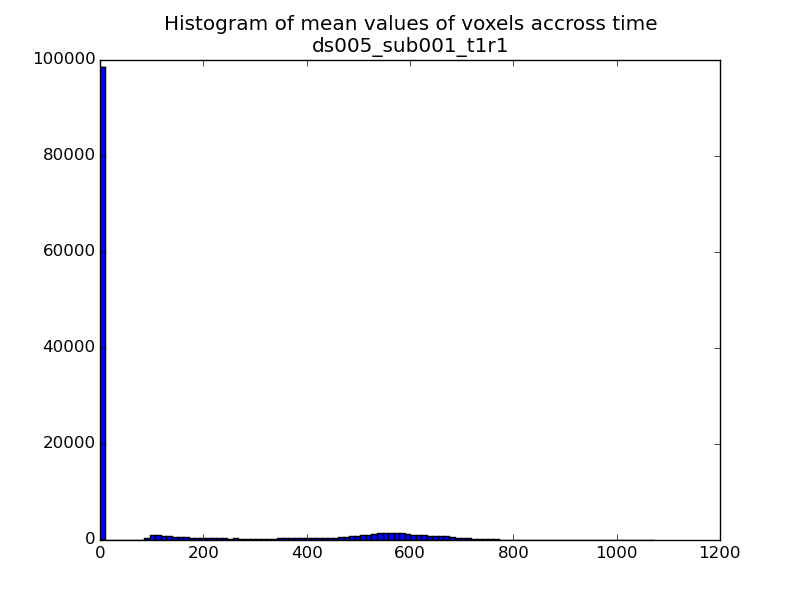
\includegraphics[width=.9\linewidth]{../fig/histograms/ds005_sub001_t1r1_hist.png}
  \caption{Subject 1}
  \label{fig:hista}
\end{subfigure}%
\begin{subfigure}{.5\textwidth}
  \centering
  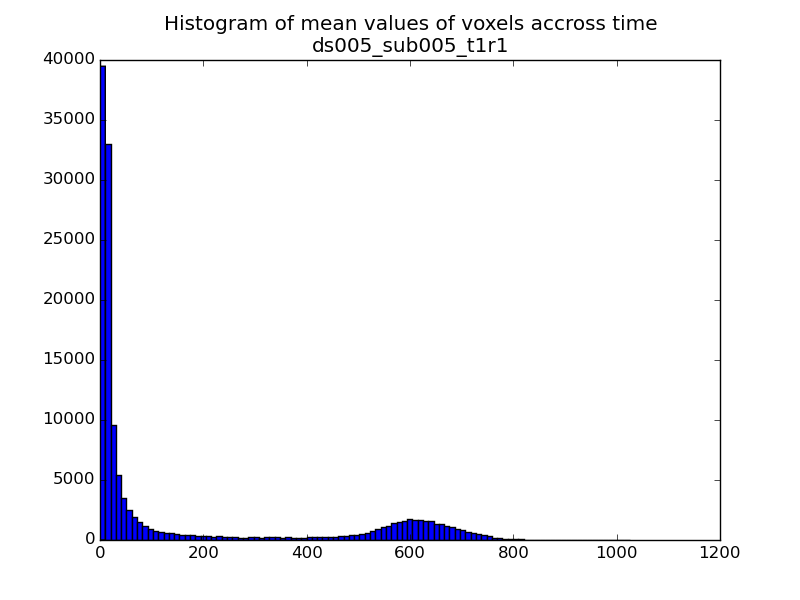
\includegraphics[width=.9\linewidth]{../fig/histograms/ds005_sub005_t1r1_hist.png}
  \caption{Subject 5}
  \label{fig:histb}
\end{subfigure}
\caption{Histogram of mean value of the voxels accross time for subject 1 and 5 - run 1}
\label{fig:hist}
\end{figure}

\par We can see from Figure \ref{fig:hista} and \ref{fig:histb} for the first run for
subjects 1 and 5 that we can set the threshold to a mean value of the voxels accross
time of 375. Our further analysis with the raw data uses a mask on the mean data accross
time that select the ones with a higher value than the threshold.

\par For the filtered data, we applied the mask provided by the Montreal Neurological 
Institute's website. The filter has 1 for the voxels inside the brain and 0 outside.
We created a function in the 'project-epsilon/code/utils/scripts' directory to 
apply the mask on these provided filtered data. The function alsoe saves a .nib file in
the same directory as the filtered data.

